\section{Brownsche Bewegung}

In diesem Versuch wird der Diffusionskoeffizient $D$ der dielektrischen Kugeln im Medium bestimmt. Dazu wird die Flüssigkeit, die die dielektrischen Kugeln enthält, mit destilliertem Wasser verdünnt auf einen Objektträger aufgebracht.
Dieser wird dann unter der Kamera platziert und so justiert, dass er sich in der Fokusebene des Lasers befindet. Dann werden einige Aufnahmen von jeweils ca. $\SI{1}{\minute}$ Länge gemacht, auf denen die Bewegung der Kugeln zu sehen ist.
Diese Bewegung wird schließlich mit Hilfe eines Computerprogramms ausgewertet. Aus dem Zusammenhang $<r^{2}>(t)>=4Dt$ (s. Vorbereitung) lässt sich nun per linearer Regression der Diffusionskoeffizient bestimmen.

Da das Computerprogramm leider nur schlecht funktionierte mussten wir mehrmals neue Aufnahmen machen. Unter den sieben Messreihen, die analysiert werden konnten, befinden sich nur drei, bei denen das Teilchen nicht stationär war (s. Abb. \ref{fig:brown_einzeln}).

\begin{figure}[tb]
	\centering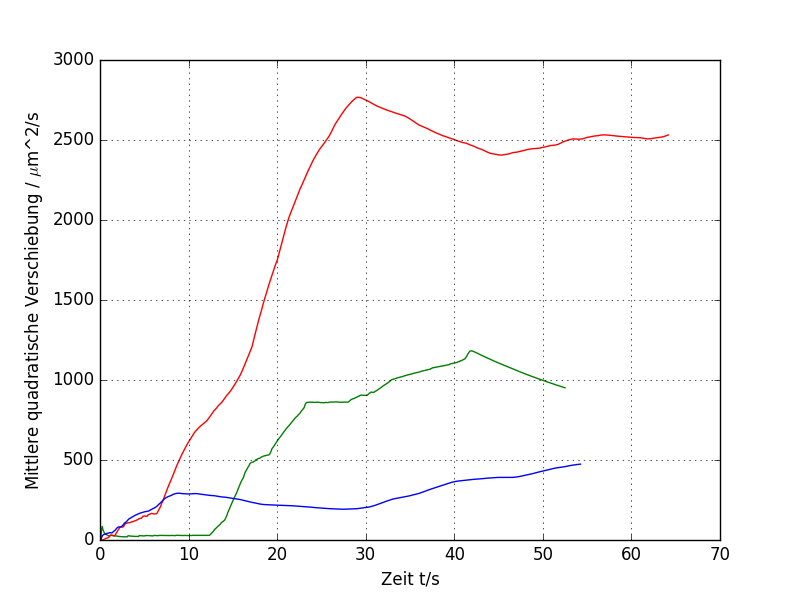
\includegraphics[width=0.7\textwidth]{fig/brown_einzeln.png}
	\caption{Mittlere quadratische Verschiebung der dielektrischen Kugeln in Abhängigkeit von der Zeit. Drei Messreihen.}
	\label{fig:brown_einzeln}
\end{figure}

\begin{figure}[tb]
	\centering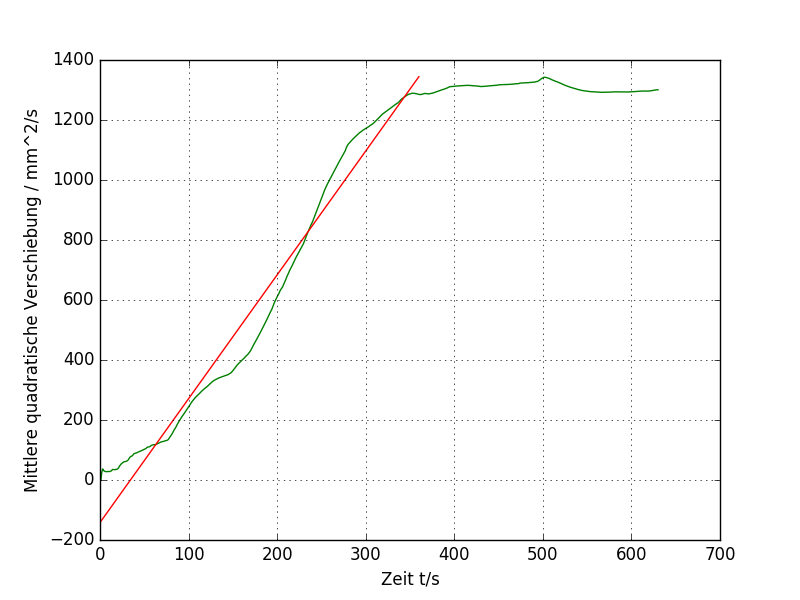
\includegraphics[width=0.7\textwidth]{fig/brown_summe.png}
	\caption{Mittlere quadratische Verschiebung der dielektrischen Kugeln in Abhängigkeit von der Zeit. Durchschnitt der Messreihen und lineare Regression zur Bestimmung von $D$.}
	\label{fig:brown_summe}
\end{figure}

Aus diesen drei Messreihen wurde der Mittelwert gebildet und eine lineare Regression im linearen Bereich der Kurve durchgeführt (s. Abb. \ref{fig:brown_summe}). Dazu wurde ``QtiPlot'' verwendet.
Die Regression der Form $<r^{2}>(t)>=At+B$ ergibt
\begin{align}
 A &= \SI{49,5\pm0,4}{\micro\meter\squared\per\second}, \\
 B &= \SI{-142\pm8}{\micro\meter\squared}.
\end{align}
Daraus ergibt sich
\begin{equation}
 D = \frac{A}{4} = (12,4\pm0,1)\cdot 10^{-12}\si{\meter\squared\per\second}.
\end{equation}
Für die systematische Unsicherheit ergibt sich durch Fehlerfortpflanzung mit $\Delta r=\SI{0,1}{\micro\metre}$ (abgeschätzt)
\begin{equation}
 \Delta D= \SI{1,3e-12}{\meter\squared\per\second}.
\end{equation}
Also insgesamt
\begin{equation}
 D = (12,4\pm0,1\pm1,3)\cdot 10^{-12}\si{\meter\squared\per\second}.
\end{equation}


\section{Maximale Fangkraft}

Aus dem Diffusionskoeffizienten und der Maximalgeschwindigkeit, mit der gefangene Kugeln bewegt werden können, lässt sich die maximale Fangkraft des Lasers bestimmen. Es gilt (s. Vorbereitung)
\begin{equation}
 F_{\textrm{T}} = \frac{k_{\textrm{B}}T}{D} v_{\textrm{max}}.
\end{equation}

Die Messung der Geschwindigkeit ergibt: bei $v=\SI{31}{\micro\meter\per\second}$ ist die Kugel gefangen, bei $v=\SI{32}{\micro\meter\per\second}$ lässt sie sich nicht mehr mitnehmen. Daraus ergibt sich
\begin{equation}
 v_{\textrm{max}} = \SI{31,5\pm0,5}{\micro\meter\per\second}.
\end{equation}

Mit $T=\SI{300}{\kelvin}$ folgt
\begin{equation}
 F_{\textrm{T}} =  \SI{1,05e-2}{\pico\newton}.
\end{equation}
Die statistische Unsicherheit ergibt sich durch die statistische Unsicherheit von $D$, $\sigma_{D}$. Per gaussscher Fehlerfortpflanzung folgt
\begin{equation}
 \sigma_{F_{\textrm{T}}} = \SI{0,02e-2}{\pico\newton}.
\end{equation}
Die systematische Unsicherheit setzt sich zusammen aus der Unsicherheit von $T$, der Unsicherheit von $v_{\textrm{max}}$ und der Unsicherheit von $D$. Es wird abgeschätzt: $\Delta T = \SI{5}{\kelvin}$.
Es ergibt sich
\begin{equation}
 \Delta F_{\textrm{T}} = \SI{0,11e-2}{\pico\newton}.
\end{equation}
Also insgesamt
\begin{equation}
 F_{\textrm{T}} = (1,05\pm0,02\pm0,11)\cdot 10^{-2} \si{\pico\newton}.
\end{equation}

Dies ist etwas geringer als der erwartete Wert im Bereich von einigen $\si{\pico\newton}$.

\section{Farbstoffe im Fokus des Lasers}

In diesem Versuchsteil wurde ein Objektträger mit rotem und schwarzem Edding bemalt und in die Fokusebene des Lasers gebracht. 
Es konnte beobachtet werden, dass auf der roten Seite des Objektträgers der Laserstrahl eine Spur hinterließ, sodass mit dem Laser "gemalt" werden konnte. Nach Anweisung des Betreuers wurde dies nur auf der roten Seite durchgeführt, auf der schwarzen Seite wäre kein, bzw nur ein sehr schwer erkennbarer Effekt vorhanden gewesen.\\
Dies liegt daran, dass die optische Pinzette nur funktioniert, wenn das einzufangende Objekt lichtdurchlässig ist, was bei roten Farbmolekülen eher der Fall ist als bei schwarzen Farbpigmenten, die das Licht nahezu komplett absorbieren.
Die Linie entsteht dadurch, dass rote Farbpigmente bis zu einem Grenzgradienten des gaußverteilten Lasers in die Mitte des Laserstrahls gezogen werden und dort einen dickeren Punkt bilden, allerdings außerhalb dieses Bereiches nach außen gedrückt werden (vgl. \ref{sec:gradient}), wodurch sich bei Bewegung des Lasers über den Objektträger eine Linie bildet.